\documentclass[border=10pt]{standalone}

\usepackage{tikz}
\usepackage{tikzsymbols}
\usetikzlibrary{calc,patterns,shapes.geometric}

\def\centerarc[#1](#2)(#3:#4:#5){\draw[#1] ($(#2)+({#5*cos(#3)},{#5*sin(#3)})$) arc (#3:#4:#5);}

\begin{document}
	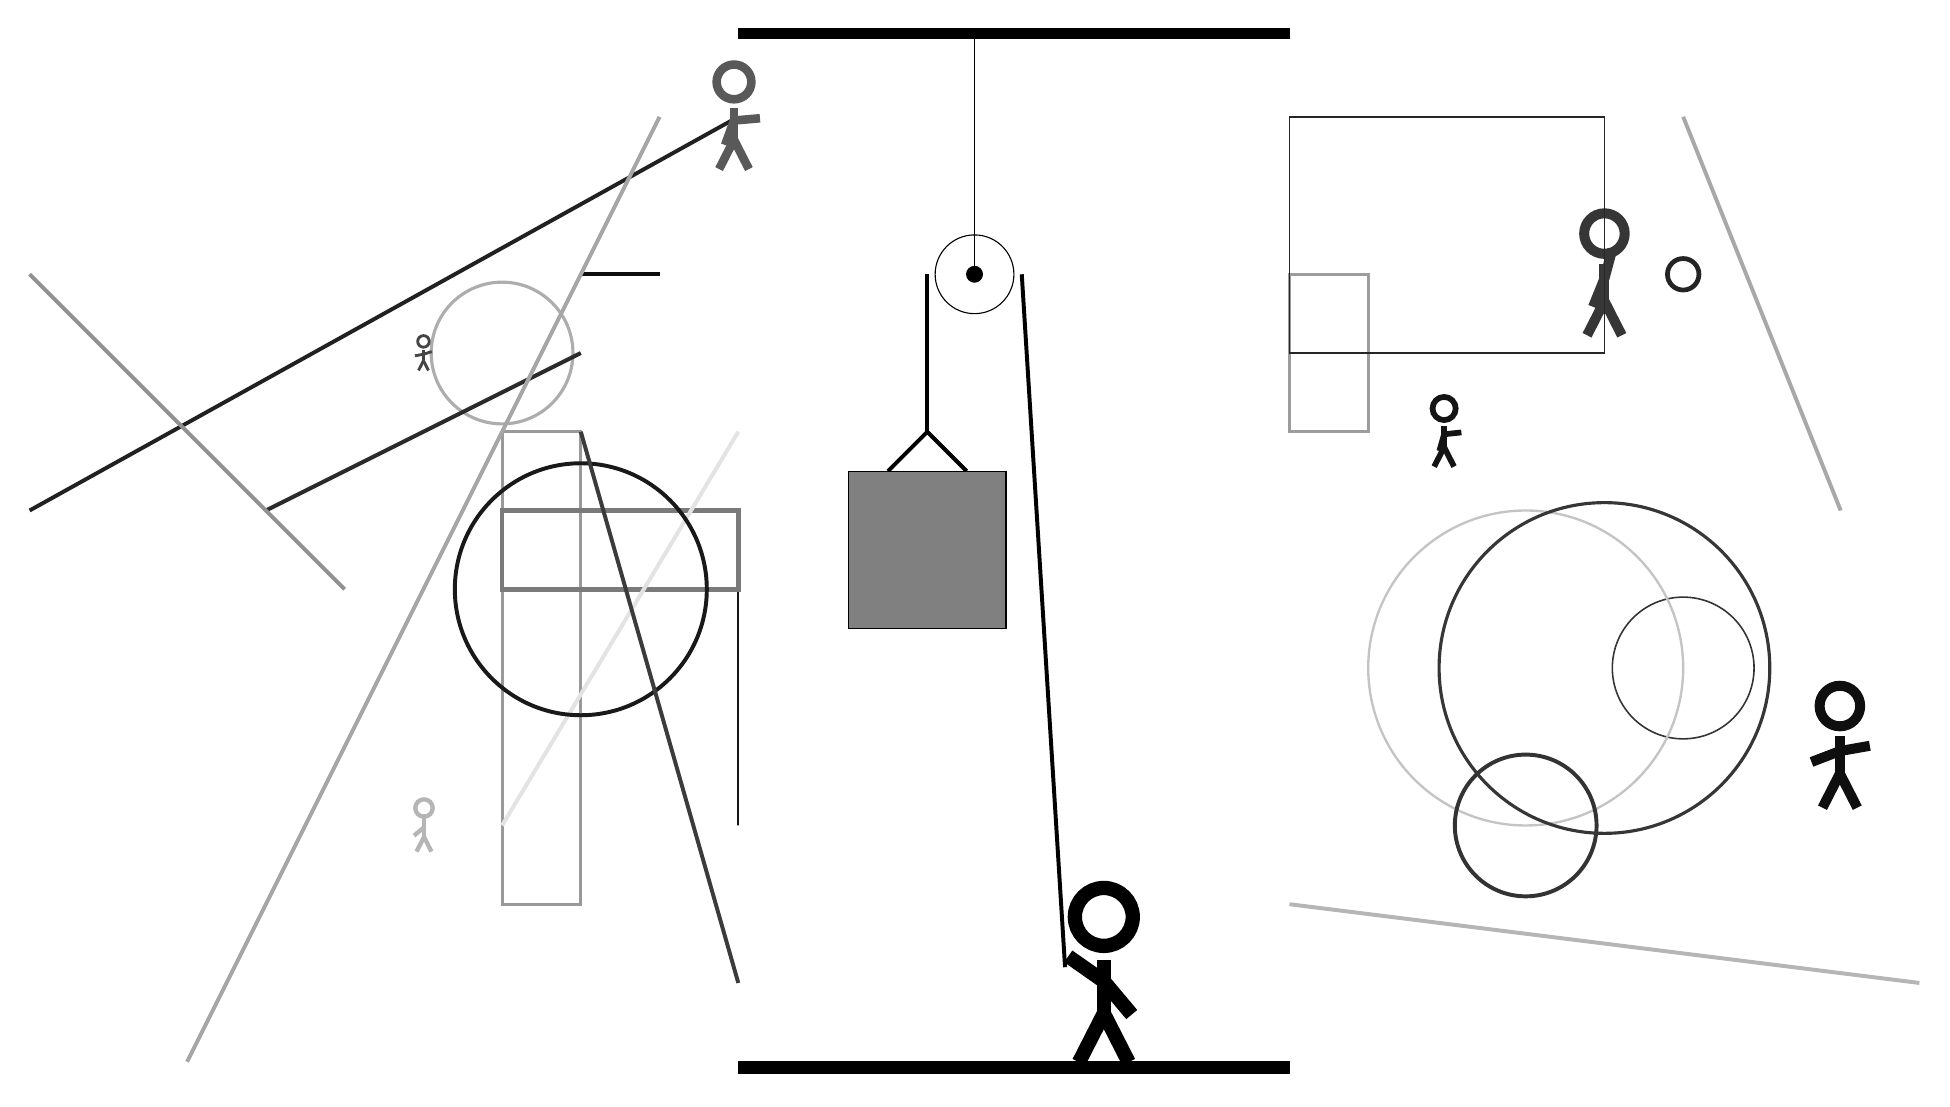
\begin{tikzpicture}
		%%%%% START %%%%%
		
		\draw[fill=black] (-2, 10) rectangle (5, 10.125);
		
		\draw (1, 7) circle (0.5);
		\draw[fill=black] (1, 7) circle (0.1);
		\draw (1, 10) -- (1, 7);
		
		\draw[line width=0.5mm] (-0.1, 4.5) -- (0.4, 5.0) -- (0.9, 4.5);
		\draw[fill=black!50] (-0.6, 4.5) rectangle (1.4, 2.5);
		
		\draw[line width=0.4mm, color=black!40] (-4, -1) rectangle (-5, 5);
		
		\draw [line width=0.2mm, color=black!80](10, 2) circle (0.9);
		\draw [line width=0.3mm, color=black!23](8, 2) circle (2.0);
		\node[line width=0.6mm, color=black!94] at (12, 1) {\Strichmaxerl[7][21][10]};
		
		\node[line width=0.3mm, color=black!92] at (7, 5) {\Strichmaxerl[4][74][6]};
		\draw[line width=0.5mm, color=black!87](-2, 9) -- (-11, 4);
		\draw[line width=0.3mm, color=black!92] (-2, 0) rectangle (-2, 4);
		\draw[line width=0.5mm, color=black!34](10, 9) -- (12, 4);
		\draw [line width=0.6mm, color=black!86](10, 7) circle (0.2);
		\draw[line width=0.6mm, color=black!52] (-2, 3) rectangle (-5, 4);
		
		\draw[line width=0.5mm, color=black!95](-4, 7) -- (-3, 7);
		\draw[line width=0.5mm, color=black!11](-5, 0) -- (-2, 5);
		\draw [line width=0.4mm, color=black!32](-5, 6) circle (0.9);
		
		\draw[line width=0.4mm, color=black!39] (6, 5) rectangle (5, 7);
		\draw [line width=0.5mm, color=black!90](-4, 3) circle (1.6);
		\node[line width=0.7mm, color=black!79] at (9, 7) {\Strichmaxerl[7][68][75]};
		\draw[line width=0.2mm, color=black!85] (5, 6) rectangle (9, 9);
		
		\draw[line width=0.5mm, color=black!83](-4, 6) -- (-8, 4);
		\node[line width=0.5mm, color=black!65] at (-2, 9) {\Strichmaxerl[6][70][5]};
		\draw[line width=0.5mm, color=black!77](-2, -2) -- (-4, 5);
		\node[line width=0.3mm, color=black!73] at (-6, 6) {\Strichmaxerl[2][10][18]};
		\draw[line width=0.5mm, color=black!29](5, -1) -- (13, -2);
		
		\draw[line width=0.5mm, color=black!35](-3, 9) -- (-9, -3);
		\draw[line width=0.5mm, color=black!43](-7, 3) -- (-11, 7);
		\node[line width=0.3mm, color=black!29] at (-6, 0) {\Strichmaxerl[3][40][90]};
		
		\draw [line width=0.5mm, color=black!80](8, 0) circle (0.9);
		\draw [line width=0.4mm, color=black!79](9, 2) circle (2.1);
		
		\draw[line width=0.5mm] (0.4, 7) -- (0.4, 5.0);
		\centerarc[line width=0.5mm](1, 7)(0:180:0.6);
		\draw[line width=0.5mm](1.6, 7) -- (2.15, -1.8);
		
		\node at (2.6, -1.9) {\Strichmaxerl[10][-35][-50]};
		
		\draw[fill=black] (-2, -3) rectangle (5, -3.15);
		
		%%%%% END %%%%%
	\end{tikzpicture}
\end{document}